\section{一些示例}

\subsection{Ti\textit{k}Z 绘图示例}

\begin{figure}[htbp!]
  \centering
  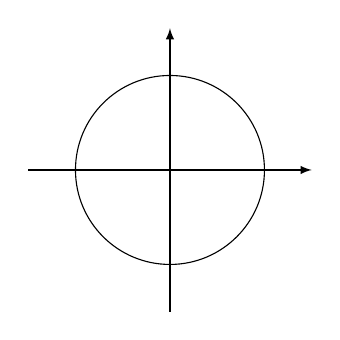
\begin{tikzpicture}[scale = 0.6]
    \draw [-latex] (-3,0) -- (3,0);
    \draw [-latex] (0,-3) -- (0,3);
    \draw (0,0) circle (2);
  \end{tikzpicture}
  \caption{这只是一个圆}
\end{figure}

\subsection{图片示例}
\begin{figure}[htbp!]
  \centering
  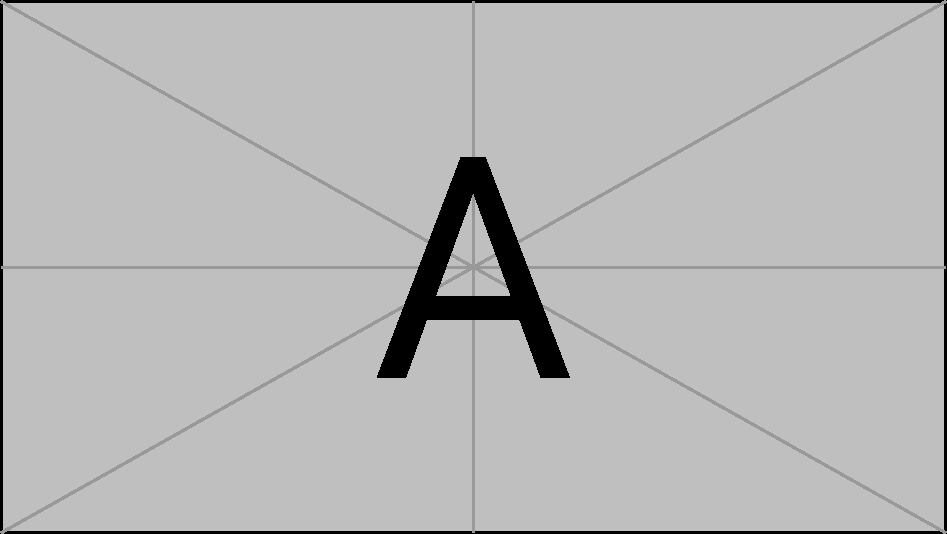
\includegraphics[scale = 0.35]{../assets/figure_a.pdf}
  \quad
  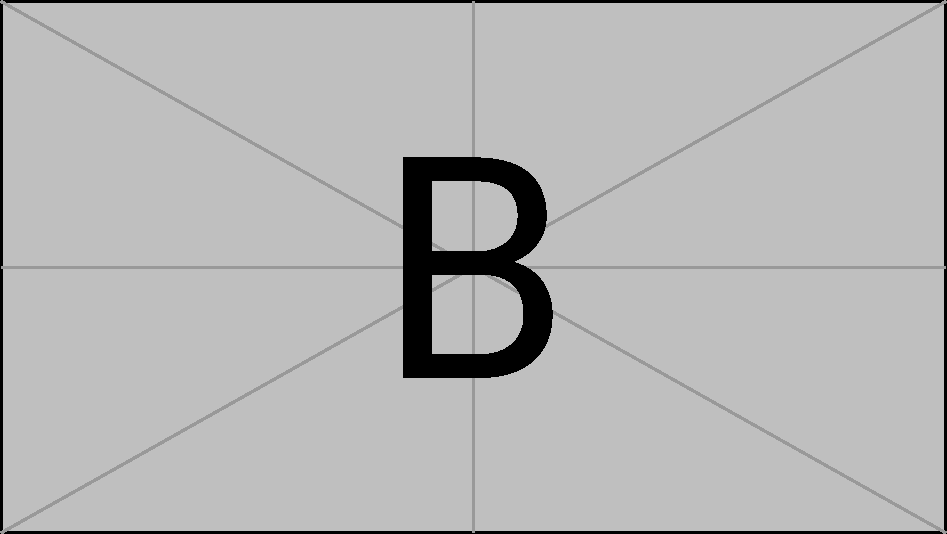
\includegraphics[scale = 0.35]{../assets/figure_b.pdf}
  \caption{这只是两张测试图片}
\end{figure}

\subsection{跨页表格示例}
\begin{longtable}{ccc}
  \caption{这只是一个长表格}                   \\
  \toprule
  姓名   & 学号        & 完成情况              \\
  \midrule
  \endfirsthead
  \multicolumn{3}{r}{\sffamily 续表 \thetable} \\
  \toprule
  姓名   & 学号        & 完成情况              \\
  \midrule
  \endhead
  \bottomrule
  \endlastfoot
  \bottomrule
  \endfoot
  姓名1  & 20201110901 & 已完成                \\
  姓名2  & 20201110902 & 已完成                \\
  姓名3  & 20201110903 & 已完成                \\
  姓名4  & 20201110904 & 已完成                \\
  姓名5  & 20201110905 & 已完成                \\
  姓名6  & 20201110906 & 已完成                \\
  姓名7  & 20201110907 & 已完成                \\
  姓名8  & 20201110908 & 摸鱼中                \\
  姓名9  & 20201110909 & 已完成                \\
  姓名10 & 20201110910 & 已完成                \\
  姓名11 & 20201110911 & 已完成                \\
\end{longtable}

\subsection{公式示例}

\subsubsection{行间公式}

\begin{equation}
  M=\sum_{k=1}^{K}m_k
\end{equation}

\begin{equation}
  \begin{aligned}
    f(x,y) & = f(0,0)+\frac{1}{1!}\left(x\diffp{}{x}+y\diffp{}{y}\right)f(0,0) \\
           & +\frac{1}{2!}\left(x\diffp{}{x}+y\diffp{}{y}\right)^2f(0,0)+K     \\
           & +\frac{1}{n!}\left(x\diffp{}{x}+y\diffp{}{y}\right)^xf(0,0)+K
  \end{aligned}
\end{equation}

\subsubsection{行内公式}

这是一个普通的行内公式 $M=\sum_{k=1}^{K}m_k$.

\subsection{代码片段示例}
\inputcode{hello.cpp}{../snippets/hello.cpp}

\newpage
